\section{Auswertung}
Im folgenden Kapitel werden die Messergebnisse der vorhandenen WebService Implementierung und der modifizierten Version mit Base64-Encoding verglichen. 
Dazu wird zuerst die Testumgebung sowie die Einstellungen die wir vorgenommen haben vorgestellt auf der wir die Implementierungen ausgef\"uhrt haben. 

\subsection{Testumgebung}
Dieser Abschnitt soll die Umgebung in Einstellungen mit denen wir die Implementierungen gegeneinander getestet haben beschreiben.\\
Die Testsysteme waren 3 Computer mit folgenden Spezifikationen:

\begin{description}
\item[CPU] Intel® Core™ i7-6700K CPU @ 4.00GHz × 8 
\item[GPU] GeForce GTX 1080
\item[RAM] 31.2 GiB
\item[OS] Ubuntu 16.04 TLS
\end{description}

F\"ur alle Tests wurden die gleichen Bilder genutzt: (horse\_left\_886x818.raw, horse\_right\_886x818.raw) in 3 unterschiedlichen Aufl\"osungen
 (100\%, 70\%, 30\%).Bei 100\% und 30\% Aufl\"osung wurde die Fenstergr\"oße 15x15 und TauMax von 40 gew\"ahlt. 
 Um zu pr\"ufen wie der Einfluss der Fenstergr\"o{\ss}e und des TauMax Wertes ist wurden 3 verschiedene Kobinationen f\"ur die Aufl\"osung 70\% gew\"ahlt:\\

\begin{description}
\item[Settings A:] Tau 20 - Fenster 7x7
\item[Settings B:] Tau 40 - Fenster 7x7
\item[Settings C:] Tau 20 - Fenster 15x15
\end{description}

 

\subsection{Messergebnisse}
In diesem Abschnitt werden die Messergebnisse vorgestellt. 

\begin{figure}[ht] 
\centering 
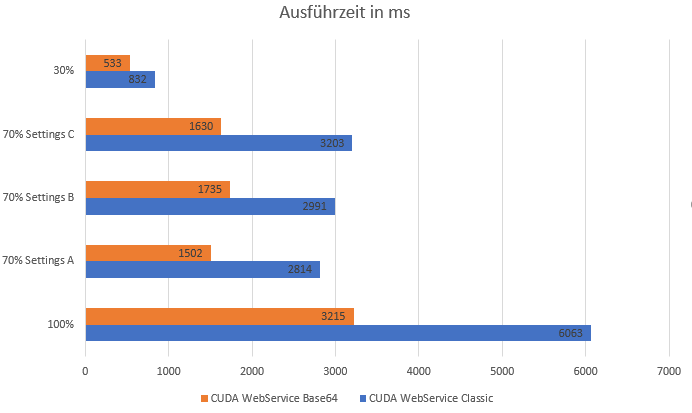
\includegraphics[scale=0.8]{Vergleich}  
\caption{Messergebnisse} 
\end{figure}

Anhand der Ergebnisse kann man sehen, dass selbst bei einer geringen Aufl\"osung des Ausgangsbildes von 30\%, 
eine Reduktion der Ausf\"uhrzeit von etwa 35\% erreicht wird, bei den h\"ohereh Aufl\"osungen sogar 42-49\%{}.
Die Base64-Implementierung kodiert und dekodiert die Rohdaten und erh\"oht deren Gr\"o\ss{}e um 33–36 \%,
dennoch ist sie fast doppelt so schnell. Das deutet darauf hin, dass der Overhead bei der Array L\"osung gr\"osser ist 
und das Parsing einzelner Bytes aufwendig.\\
M\"ochte man also nicht auf WebServices verzichten, aber trozdem eine Performance Steigerung erreichen, 
ist das \"Ubertragen eines Base64 Kodierten Strings anstatt einzelner Bytes eine Alternative die man in Betracht ziehen sollte. 